\documentclass[../../../../main.tex]{subfiles}
\begin{document}

\begin{flushright}
\footnotesize\textit{【自動文字起こし・要確認】}
\end{flushright}

\noindent
[\textbf{解}] Aの期待値は $1$ $\dots$ ①

\noindent
Bの期待値 $E(b)$ は、1回目があたるかどうかで場合分けして
\[
E(b) = 2p + p(1-p) = -p^2 + 3p \quad \dots \text{②}
\]

\noindent
Cの期待値 $E(c)$ も同様に
\[
E(c) = 3p^2 + 2p(1-p) = p^2 + 2p \quad \dots \text{③}
\]

\noindent
$0 < p < 1$ と右のグラフから
\[
\begin{cases}
0 < p < \frac{3 - \sqrt{5}}{2} \text{の時} & \text{A} \\
p = \frac{3 - \sqrt{5}}{2} \text{の時} & \text{A, B} \\
\frac{3 - \sqrt{5}}{2} < p < \frac{1}{2} \text{の時} & \text{B} \\
p = \frac{1}{2} \text{の時} & \text{B, C} \\
\frac{1}{2} < p < 1 \text{の時} & \text{C}
\end{cases}
\]

\begin{center}
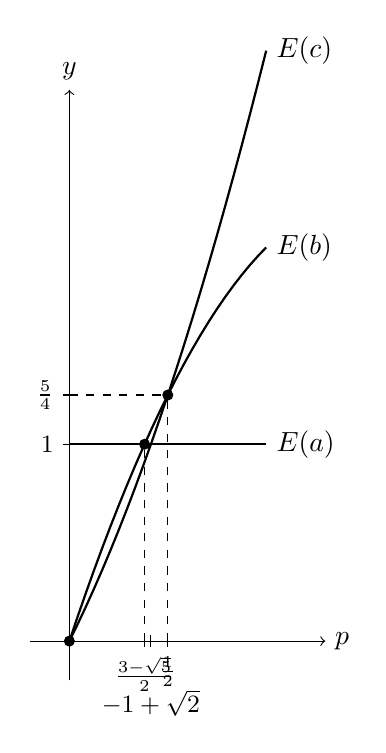
\begin{tikzpicture}[scale=2.5]
    % Axes
    \draw[->] (-0.2,0) -- (1.3,0) node[right]{$p$};
    \draw[->] (0,-0.2) -- (0,2.8) node[above]{$y$};
    
    % Key x ticks
    \draw (0.382,0.03) -- (0.382,-0.03) node[below, font=\small]{$\frac{3-\sqrt{5}}{2}$};
    \draw (0.5,0.03) -- (0.5,-0.03) node[below, font=\small]{$\frac{1}{2}$};
    \draw (0.414,0.03) -- (0.414,-0.03) node[below, font=\small, yshift=-12pt]{$-1+\sqrt{2}$};
    
    % Key y ticks
    \draw (0.03,1) -- (-0.03,1) node[left, font=\small]{1};
    \draw (0.03,1.25) -- (-0.03,1.25) node[left, font=\small]{$\frac{5}{4}$};
    
    % Curves
    % E(a) = 1
    \draw[thick, domain=0:1] plot (\x, 1) node[right]{$E(a)$};
    
    % E(b) = -p^2 + 3p
    \draw[thick, domain=0:1] plot (\x, {-\x*\x + 3*\x}) node[right]{$E(b)$};
    
    % E(c) = p^2 + 2p
    \draw[thick, domain=0:1] plot (\x, {\x*\x + 2*\x}) node[right]{$E(c)$};
    
    % Intersections / dashed lines
    \draw[dashed] (0.382,0) -- (0.382,1);
    \draw[dashed] (0.5,0) -- (0.5,1.25);
    \draw[dashed] (0,1.25) -- (0.5,1.25);
    
    \fill (0.382,1) circle (0.8pt);
    \fill (0.5,1.25) circle (0.8pt);
    \fill (0,0) circle (0.8pt);
\end{tikzpicture}
\end{center}

\end{document}
